\chapter{Q07}
\emph{Q7: Explain the basic two approaches for error control in WSNs. What are
the pros and cons of each approach?}

\section{Error Control}

\begin{description}
	\item{Error-free} deliver exactly the sent bits/packets
	\item{In-sequence} deliver them in the original order
	\item{Duplicate-free} and at most once
	\item{Loss-free} and at least once
\end{description}


\section{Backward-errorcontrol - ARQ: Reactive}

Header information

Checksum Cyclic redundancy check (CRC) 

Feedback from receiver to sender ACK or NACK

Timeout on ACK for retransmitting

Maximum number of retransmission attempts?

\subsection{Standard ARQ protocols}
\begin{description}
	\item Stop-and-Wait
	\item Go-back-N
	\item Selective Repeat
\end{description}

\section{Forward error control - FEC: Proactive}

Add additional redundancy in a packet

\begin{center}
 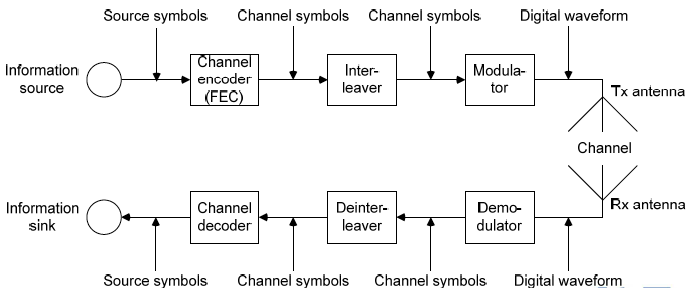
\includegraphics[scale=0.5]{img/ErrorControle-FEC.png}
\end{center}

\subsection{FEC Cost}

\begin{description}
\item Encoding/Decoding (energy + latency)
\item Tx/Rx longer packets (energy + latency)
\end{description}

